\documentclass[fullscreen=true, unicode, bookmarks=false]{beamer}

\usepackage{lmodern}

\usepackage[T2A]{fontenc} 
\usepackage[UTF8]{inputenc}
\usepackage[russian]{babel}
\usepackage{amsmath,amsfonts,amssymb}
\usepackage[export]{adjustbox}
\usepackage{textgreek}
\sloppy

\setbeamertemplate{navigation symbols}{}

\usetheme{Madrid}

\usecolortheme{whale}

\usefonttheme{professionalfonts} % default family is serif

\setbeamertemplate{footline}{\hspace*{.5cm}\scriptsize{\insertshorttitle
\hspace*{50pt} \hfill\hspace*{.5cm}}\vspace{5pt}} 

\setbeamercolor{bibliography entry author}{fg=black}

\title[]{ Колебательное рождение пространственно-неоднородных режимов в одной краевой задаче с отклонением }   
\author[]{{\large Леонид Ивановский}} 
\date{}
\institute[]

\begin{document}

\begin{frame}
\titlepage
\end{frame} 

\begin{frame}
\frametitle{ Краевая задача }
 
\begin{equation}\label{ivanovsky-eq1}
	u' = d \ddot{u} - \gamma u + F(u),
\end{equation}	
	
$$  u'\mid_{x=0} \, = 0, $$
$$ u'\mid_{x=1} \, = \alpha\,u\mid_{x=x_0}. $$

$$ \alpha, \gamma \in \mathbb{R}, \quad d > 0, \quad x_0 \in [0, 1]. $$

\end{frame}

\begin{frame}
\frametitle{ Замены }
	
$$ t_1 = d \times t, $$

\bigskip

$$ u(x, t) = w(x)\,\mbox{exp}\left( \lambda - \frac{\gamma}{d}t \right). $$

\end{frame}

\begin{frame}
	
\begin{equation}\label{ivanovsky-eq2}
	w'' - \lambda w = 0,
\end{equation}

$$ w'(0) = 0, $$
$$ w'(1) = \alpha\,w(x_0). $$

\end{frame}

\begin{frame}
\frametitle{ Краевые условия }
	
$$ x = 1: $$

\bigskip

$$ \mu \sh \mu = \alpha \ch(\mu x_0) $$

\bigskip

$$ \mu^2 = \lambda. $$

\end{frame}

\begin{frame}
	
$$ \mu = \pm i \omega $$

\bigskip

\begin{equation}\label{ivanovsky-eq3}
	g(\omega) - \alpha = 0
\end{equation}

\bigskip

$$ g(\omega) = -\frac{\omega \sin \omega}{\cos \omega x_0}. $$

\end{frame}

\begin{frame}
\frametitle{ Метод исследования } 

\begin{figure} 

\includegraphics[scale=0.25]{python.png}  
\hfill

\includegraphics[scale=0.6]{openmp.jpg} 
\end{figure}

\end{frame}

\begin{frame}
\frametitle{ Метод исследования } 

\begin{figure}
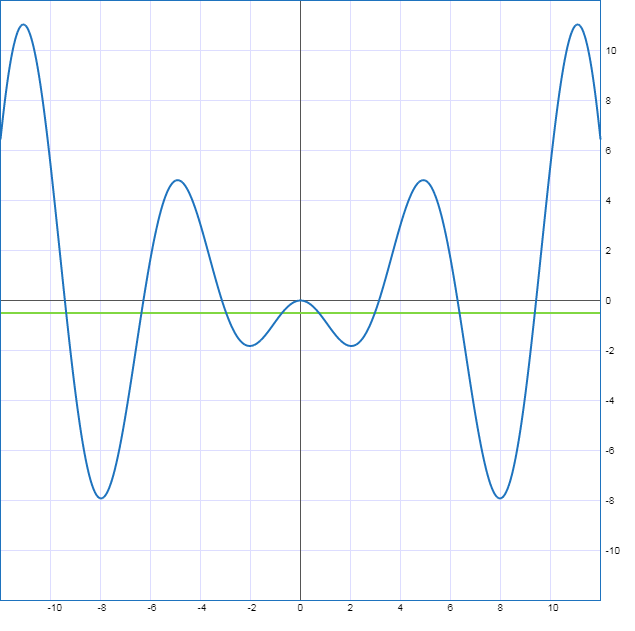
\includegraphics[scale=0.37]{xsinx.png} 
\end{figure}

\end{frame}

\begin{frame}
\frametitle{ Результаты исследования } 

{\tiny  $$ x_0 = 0.0 $$}
\vspace{-0.8cm}
\begin{figure}
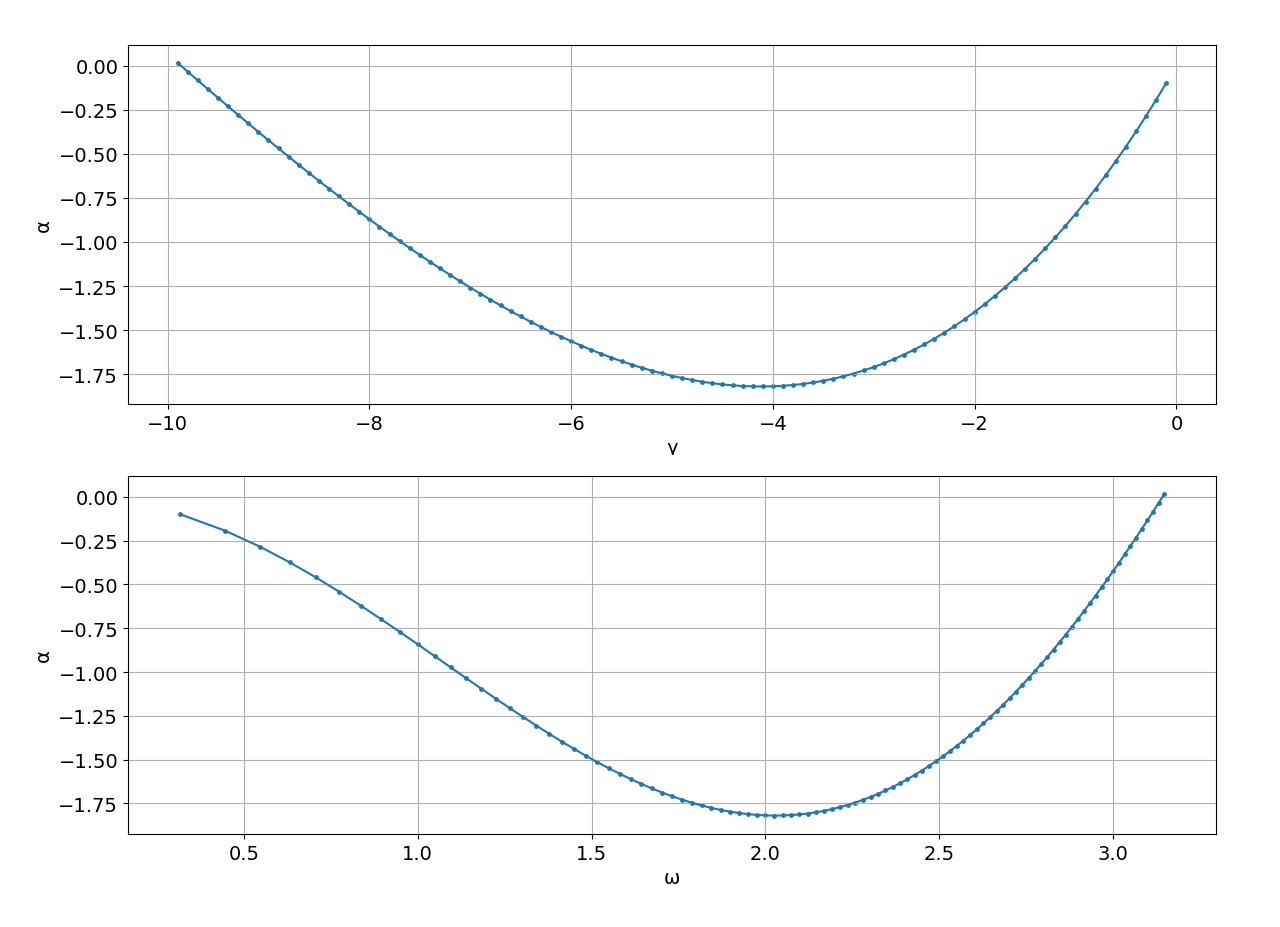
\includegraphics[scale=0.35]{0,0.png} 
\end{figure}

\end{frame}

\begin{frame}
\frametitle{ Результаты исследования } 

{\tiny  $$ x_0 = 0.4 $$}
\vspace{-0.8cm}
\begin{figure}
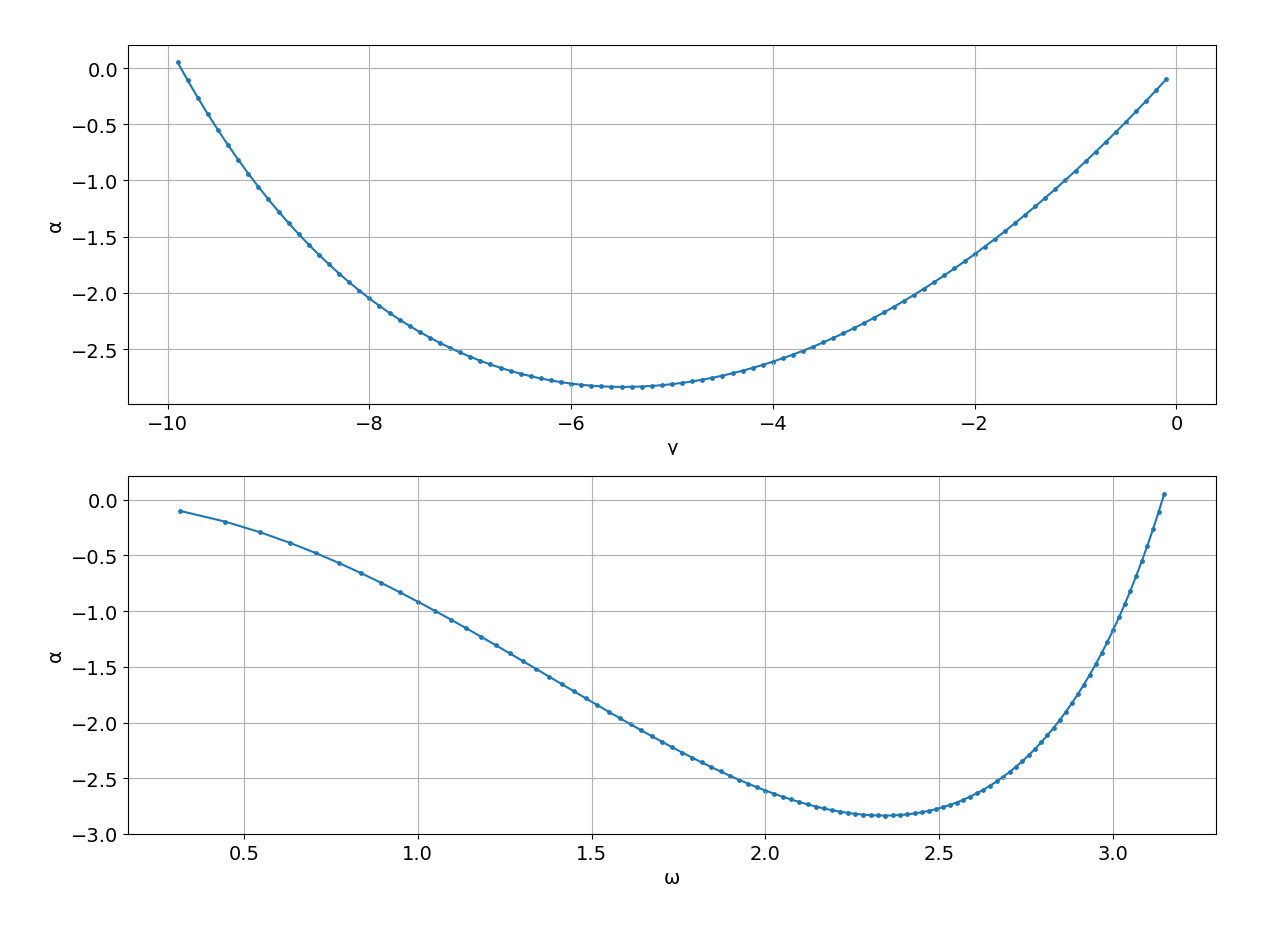
\includegraphics[scale=0.35]{0,4.png} 
\end{figure}

\end{frame}

\begin{frame}
\frametitle{ Результаты исследования } 

{\tiny  $$ x_0 = 0.495 $$}
\vspace{-0.8cm}
\begin{figure}
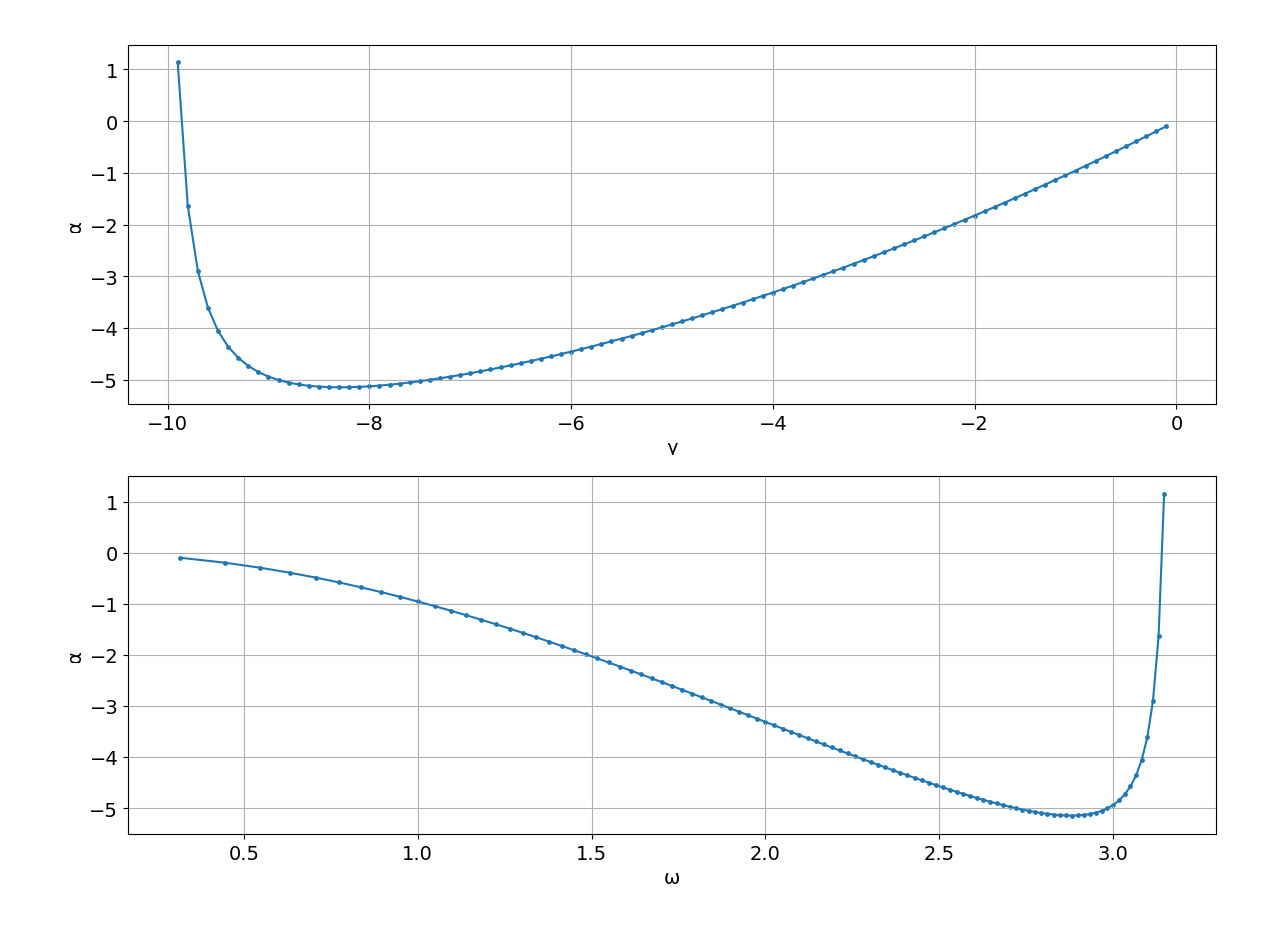
\includegraphics[scale=0.35]{0,495.png} 
\end{figure}

\end{frame}

\begin{frame}
\frametitle{ Результаты исследования } 

{\tiny  $$ x_0 = 0.51 $$}
\vspace{-0.8cm}
\begin{figure}
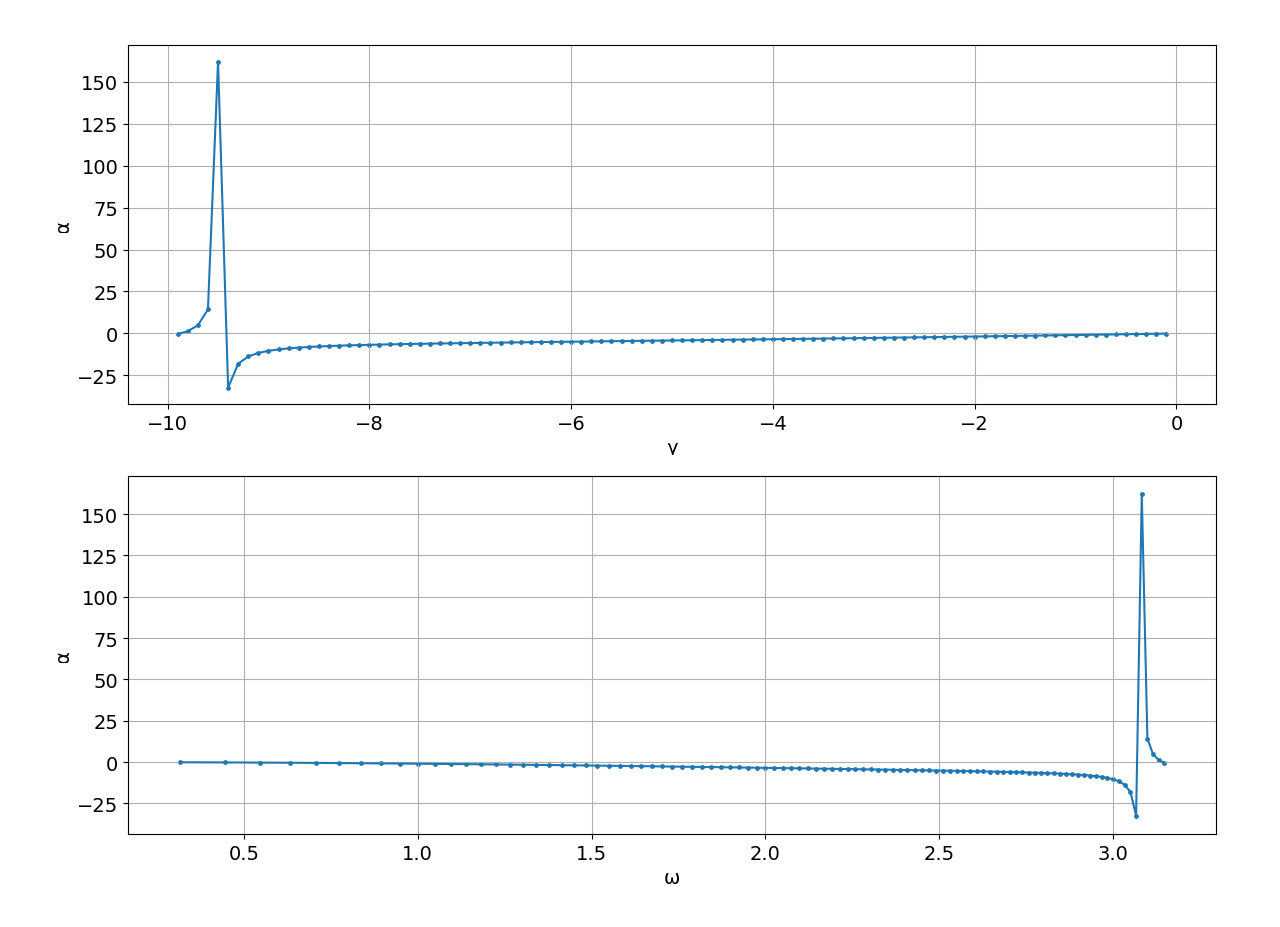
\includegraphics[scale=0.35]{0,51.png} 
\end{figure}

\end{frame}

\begin{frame}
\frametitle{ Результаты исследования } 

{\tiny  $$ x_0 = 0.66 $$}
\vspace{-0.8cm}
\begin{figure}
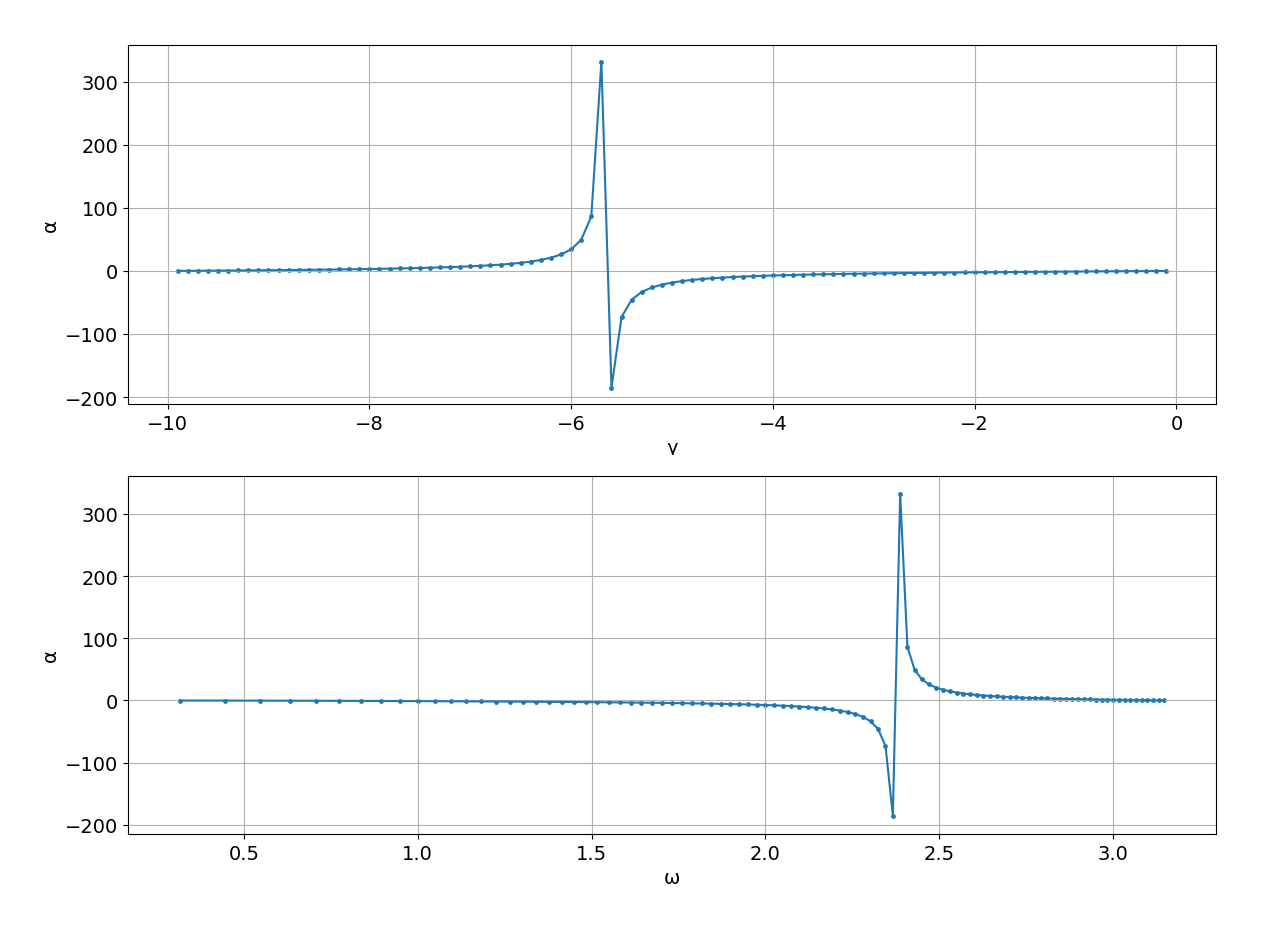
\includegraphics[scale=0.35]{0,66.png} 
\end{figure}

\end{frame}

\end{document}